\documentclass{book}
\title{Estructura de datos - UFM}
\author{David Gabriel Corzo Mcmath}
\date{2020-Jan-06 07:08:59}
%%%%%%%%%%%%%%%%%%%%%%%%%%%%%%%%%%%%%%%%%%%%%%%%%%%%%%%%%%%%%%%%%%%%%%%%%%%%%%%%%%%%%%%%%%%%%%%%%%%%%%%%%%%%%%%%%%%%%%%%%%%%%%%%%%%%%%%%%%%%%%%
\usepackage[margin = 1in]{geometry}
\usepackage{graphicx}
\usepackage{fontenc}
\usepackage{pdfpages}
\usepackage[spanish]{babel}
\usepackage{amsmath}
\usepackage{amsthm}
\usepackage[utf8]{inputenc}
\usepackage{enumitem}
\usepackage{mathtools}
\usepackage{import}
\usepackage{xifthen}
\usepackage{pdfpages}
\usepackage{transparent}
\usepackage{color}
\usepackage{fancyhdr}
\usepackage{lipsum}
\usepackage{sectsty}
\usepackage{titlesec}
\usepackage{calc}
\usepackage{lmodern}
\usepackage{xpatch}
\usepackage{blindtext}
\usepackage{bookmark}
\usepackage{fancyhdr}
\usepackage{xcolor}
\usepackage{tikz}
\usepackage{blindtext}
\usepackage{hyperref}
\usepackage{listing}
\usepackage{spverbatim}
\usepackage{fancyvrb}
\usepackage{fvextra}
\usepackage{amssymb}
\usepackage{pifont}
\usepackage{longtable}
\usetikzlibrary{shapes,arrows}
%%%%%%%%%%%%%%%%%%%%%%%%%%%%%%%%%%%%%%%%%%%%%%%%%%%%%%%%%%%%%%%%%%%%%%%%%%%%%%%%%%%%%%%%%%%%%%%%%%%%%%%%%%%%%%%%%%%%%%%%%%%%%%%%%%%%%%%%%%%%%%%
\begin{document}
\maketitle
\tableofcontents

% Begin block styles
\tikzstyle{decision}=[diamond, draw, fill=white!20,text width=4.5em, text badly centered, node distance=3cm, inner sep=0pt]
\tikzstyle{block}=[rectangle, draw, fill=white!20,text width=5em, text centered, rounded corners, minimum height=4em]
\tikzstyle{line}=[draw, -latex']
\tikzstyle{cloud}=[draw, ellipse,fill=white!20, node distance=3cm,minimum height=2em]
% End block styles 


\chapter{Clase introductoria - 2020-01-06}
\section{Conceptos fundamentales}
\begin{itemize}
    \item Activos: Es lo que yo tengo derecho de.
    \item Pasivos: Son aquellas obligaciones que tengo que incurrir.
    \item Patrimonio: Todo lo que le pertenece a la empresa, es el capital; el pasivo + capital cuadra con el activo. El capital no solo es dinero. 
    \item Ingreso o ventas: todos los beneficios que se derivan por la actividad de vender, los ingresos pueden ser 
    \item Costos y gastos: Costos es lo que me cuesta hacer un producto, los gastos es lo que me cuesta venderlo, es todo el gasto adicional que realiza para realizar sus operaciones.
\end{itemize}

%%%%%%%%%%%%%%%%%%%%%%%%%%%%%%%%%%%%%%%%%%%%%%%%%%%%%%%%%%%%%%%%%%%%%%%%%%%%%%%%%%%%%%%%%%%%%%%%
\subsection{Ejemplo}
\[
  \text{Activo} = \text{Pasivo} (+) \text{Capital} 
\]

\subsection{Activos}
\begin{itemize}
    \item Corrientes: son los que se pueden liquidar a \textbf{corto} plazo a efectivo.
        \begin{itemize}
            \item Disponibles 
            \item Exigibles
        \end{itemize}
    \item No corrientes: son los que se liquidan a \textbf{largo} plazo a efectivo. 
        \begin{itemize}
            \item Realizables
            \item fijos 
        \end{itemize}
\end{itemize}

%%%%%%%%%%%%%%%%%%%%%%%%%%%%%%%%%%%%%%%%%%%%%%%%%%%%%%%%%%%%%%%%%%%%%%%%%%%%%%%%%%%%%%%%%%%%%%%%
\subsection{Pasivos}
\begin{itemize}
    \item Corrientes:
        \begin{itemize}
            \item Bancos: Un prestamo, una hipotéca, carta de crédito.
            \item Proveedores: las obligaciones incurridas por el inventario que yo debo.
            \item Gastos acumulados por pagar: son pagos que se acumulan a través del tiempo.
            \item Prestaciones laborales: pagos adicionales que establece la ley a sus empleados, el bono 14 o el aguinaldo.
            \item Provisión para indemnización: La reserva para cuando los empleados son despedidos y tienen que ser pagados por indemnización.
        \end{itemize}
\end{itemize}


%%%%%%%%%%%%%%%%%%%%%%%%%%%%%%%%%%%%%%%%%%%%%%%%%%%%%%%%%%%%%%%%%%%%%%%%%%%%%%%%%%%%%%%%%%%%%%%%
\subsection{Patrimonio}
\begin{itemize}
    \item Capital - Aportaciones: en aportaciones lo que los accionistas aportan a la sociedad.
    \item Utilidades retenidas: se retiene el 5\% del dinero de los años anteriores.
        \begin{itemize}
            \item Reserva legal: aquellas reservas de dinero que debo tener por ley, es obligatorio no es voluntario como las reservas estatuarias.
            \item Reservas estatutarias: hacer reservas a favor de los empleados; ejemplo que el 10\% lo voy a separar para futuros proyectos.
            \item Resultados acumulados: las ganancias de los aos anteriores o pérdidas, la suma de todo.  
        \end{itemize}
\end{itemize}

%%%%%%%%%%%%%%%%%%%%%%%%%%%%%%%%%%%%%%%%%%%%%%%%%%%%%%%%%%%%%%%%%%%%%%%%%%%%%%%%%%%%%%%%%%%%%%%%
\subsection{Ingresos}
\begin{itemize}
    \item Ventas: por ventas.
    \item Intereses ganados: como los intereses por bancos.
    \item Otros ingresos: se venden activos por arriba de su precio de depreciación.
\end{itemize}

%%%%%%%%%%%%%%%%%%%%%%%%%%%%%%%%%%%%%%%%%%%%%%%%%%%%%%%%%%%%%%%%%%%%%%%%%%%%%%%%%%%%%%%%%%%%%%%%
\subsection{Gastos}
\begin{itemize}
    \item Costos: El costo al que yo adquirí en el inventario. 
    \item Gastos: todos los gasto que se tengan, seguridad, luz, teléfono.
    \item Otros gastos: No son usuales pero son gastos, una multa, intereses bancarios, etc. 
\end{itemize}

%%%%%%%%%%%%%%%%%%%%%%%%%%%%%%%%%%%%%%%%%%%%%%%%%%%%%%%%%%%%%%%%%%%%%%%%%%%%%%%%%%%%%%%%%%%%%%%%
\subsection{Estados financieros básicos}
\begin{itemize}
    \item Balance general: enseñar la situación de una empresa en una fecha específica. ``Balance general al <fecha>'', es como una foto de ese día.
        \begin{itemize}
            \item Ejemplo: la billetera, el balance general, tiene Q3; el balance es de 303 por 300 en efectivo y 3 en bancos.
                \begin{center}
                   \begin{tabular}{ | p{5cm} | p{5cm} | }
                       \hline
                        Activo & Pasivo     \\
                       \hline
                       Caja y bancos Q303 & -- \\ 
                       -- & Capital Q303 \\ 
                       \hline
                   \end{tabular}
                \end{center}
        \end{itemize}

    \item Estado de resultados: si la empresa está ganando o perdiendo, es un resumen de sus ingresos y sus gastos.
    \item Estado de patrimonio: mostrar las variaciones que hubieron en el capital durante un año, puede aumentar o disinuir.
    \item Estado de flujos de efectivo: todo el efectivo que se recudé en un año y dónde están invertidos. 
    \item Notas a los estados financieros: la información general que ayuda a entender sus estados financieros; como cual método de depreciación uso, clientes morosos. 
\end{itemize}

%%%%%%%%%%%%%%%%%%%%%%%%%%%%%%%%%%%%%%%%%%%%%%%%%%%%%%%%%%%%%%%%%%%%%%%%%%%%%%%%%%%%%%%%%%%%%%%%
\subsection{Auditoría externa}
\begin{itemize}
    \item Es importante para comprobar que la información financiera esté registrada correctamente.
\end{itemize}

%%%%%%%%%%%%%%%%%%%%%%%%%%%%%%%%%%%%%%%%%%%%%%%%%%%%%%%%%%%%%%%%%%%%%%%%%%%%%%%%%%%%%%%%%%%%%%%%
\section{Ejercicio: ¿invertimos en la empresa o no?}
\begin{itemize}
    \item La empresa es Disney, si tenía que invertir.
\end{itemize}


\chapter{Clase introductoria - 2020-01-08}
\section{Kickoff}
\begin{itemize}
    \item 
\end{itemize}


\chapter{Clase de avance de tarea \# 2}
\section{Productividad}
\begin{itemize}
    \item Eficacia: lograr los resultados \textbf{esperados}. 
    \item Eficiencia: los que demuestran resultados \textbf{esperados} con la mínima cantidad de recursos, \textbf{exceden expectativas}.
    \item Efectividad: es el logro de la \textbf{eficiencia} sostenida a través del tiempo.
\end{itemize}

\subsection{Las estrategias mencionadas anteriormente}
\begin{itemize}
    \item Está bien cualquiera de las estrategias de productividad
\end{itemize}

%%%%%%%%%%%%%%%%%%%%%%%%%%%%%%%%%%%%%%%%%%%%%%%%%%%%%%%%%%%%%%%%%%%%%%%%%%%%%%%%%%%%%%%%%%%%%%%%
\section{Factores}
\begin{itemize}
    \item Hay factores que no puedo controlar:
        \begin{itemize}
            \item Tenemos que entender como empresarios de \textbf{disernir} qué factores controlamos y cuáles no:
                \begin{enumerate}
                    \item Económicos 
                    \item Ecológicos 
                    \item Políticos y legales 
                    \item Tecnología
                    \item Éticos 
                    \item Sociales y culturales 
                \end{enumerate}
            
            \item \emph{\textbf{Ejemplo: }Los factores externos como aquellos de un cambio de precio en la industria de transporte.}
            \item \textbf{Nos preguntamos:} ¿Se dispara el precio de la leche? las industrias que emplean la leche como derivada de su producto o como complemento de su producto.
            \item \emph{\textbf{Ejemplo: }Industria de cemento deja de producir cemento} 
        \end{itemize}
    
    \item Factores internos que puedo controlar: 
        \begin{itemize}
            \item Los puedo controlar.
            \item Estrategia: se debe saber qué tan estable es el territorio en el que se está haciendo negocios.
            \item Los países que son inestables no atraen inversión extrangera.
        \end{itemize}
\end{itemize}

%%%%%%%%%%%%%%%%%%%%%%%%%%%%%%%%%%%%%%%%%%%%%%%%%%%%%%%%%%%%%%%%%%%%%%%%%%%%%%%%%%%%%%%%%%%%%%%%
\section{Estrategia}
\begin{itemize}
    \item Steakholders:
        \begin{itemize}
            \item Son clientes, accionistas, inversionistas, proveedores, etcétera. Cualquier persona interesadas en la empresa. Es importante tener una buena relación con dichos steakholders.
        \end{itemize}
    
    \item Tendencias: 
        \begin{itemize}
            \item Pueden ser conductas, actitudes, preferencias que puedan indicar hacia donde se mueve el consumidor.
            \item Las tendencias de la demanda de los consumedores se abre una oportunidad de negocios que se deben aprovechar.
        \end{itemize}
    
    \item Conosza el entorno en el que opera su empresa: se necesita saber el entorno.
        \begin{itemize}
            \item \textbf{Nos preguntamos:} ¿qué servicios o productos vende?
            \item \textbf{Nos preguntamos:} ¿a que industria permanece?
        \end{itemize}
        
    \item \emph{\textbf{Definición de ``Industria:":} El conjunto de empresas que se dedican a un mismo grupo de productos o servicios.}
\end{itemize}

%%%%%%%%%%%%%%%%%%%%%%%%%%%%%%%%%%%%%%%%%%%%%%%%%%%%%%%%%%%%%%%%%%%%%%%%%%%%%%%%%%%%%%%%%%%%%%%%

\section{Manejan información correcta de la fuente correcta}
\begin{itemize}
    \item Las tendencias nor permiten detectar oportunidades de negocios.
    \item \emph{\textbf{Ejemplo: }China crecerá aun más, esta es una tendencia mal redactada por que no tiene cifras.}
    \item Una tendencia se manifiesta en cifras, no en declaraciones.
    \item 
\end{itemize}


\chapter{Clase }
\section{Unit testing}
\begin{itemize}
    \item 
\end{itemize}


%%%%%%%%%%%%%%%%%%%%%%%%%%%%%%%%%%%%%%%%%%%%%%%%%%%%%%%%%%%%%%%%%%%%%%%%%%%%%%%%%%%%%%%%%%%%%%%%
\section{Postman}
\begin{itemize}
 Pasos para probar un API:
        \begin{itemize}[label=$\downarrow$]
            \item New $\rightarrow$ Crear una collección.
            \item Poner el URL al API.
        \end{itemize}

%%%%%%%%%%%%%%%%%%%%%%%%%%%%%%%%%%%%%%%%%%%%%%%%%%%%%%%%%%%%%%%%%%%%%%%%%%%%%%%%%%%%%%%%%%%%%%%%
\section{Jmeter}
\begin{itemize}[label=$\downarrow$]
    \item Test plan es mi route de los tests.
    \item Add $\rightarrow$ Thread $\rightarrow$ Thread groups
    \item Basic Test $\rightarrow$ Sampler $\rightarrow$ HTTP request
        \begin{itemize}[label=$\downarrow$]
            \item Server name or IP: numbre de dominio 
            \item Numero de puerto 
        \end{itemize}
    \item Agregamos un listener:
        Basic Test $\rightarrow$ Listener $\rightarrow$ 
        
\end{itemize}


\chapter{Clase - 2020-01-20}
\section{Pricing}
\begin{itemize}
    \item \emph{\textbf{Definición de ``pricing":} son las técnicas que me permiten determinar a qué precio puedo poner mi producto, es el arte de saber comprender como cuánto un cliente estaría dispuesto a pagar por un producto o servicio, intensando obtener el máximo margen de utilidad posible de éste.}
    \item Hay una gama de dificultades que no controlamos:
        \begin{itemize}
            \item Precios de materia prima 
            \item Situación político-económica del país.
        \end{itemize}
    
    \item Hay diferentes tipos de productos:
        \begin{itemize}
            \item Los productos superfluos: son productos de lujo.
            \item Los productos necesarios: son productos que necesito.
        \end{itemize}
    
    \item Objetivos: 
        \begin{enumerate}
            \item Maximizar las ganancias: uno vende no por benevolencia, es por que quiero derivar beneficios.
            \item Aumentar los volúmenes de venta: a veces si no balanceo las unidades vendidas con el precio puedo perder.
            \item Consolidar un prestigio: tiene que ver con lealtad, si tengo un buen producto puedo elevar más el precio.
            \item Neutralizar la guerra de precios: todos pierden en una guerra de precios. 
        \end{enumerate}
    
    \item Deteminación de la estrategia de pricing:
        \begin{itemize}
            \item Lo más importante es la estrategia con el cliente.
            \item Depende del tipo de mercado que quiero llegar. 
            \item Establecer una estrategia de precios que sea compatible para el tipo de mercado al que llegaré.
            \item Hacer un estudio de mercado antes de lanzar un producto al mercado.
            \item Evaluar si se tiene capacidad de vender las unidades necesarias para sobrevivr.
            \item Controlar todos los factores.
        \end{itemize}
    
\end{itemize}



%%%%%%%%%%%%%%%%%%%%%%%%%%%%%%%%%%%%%%%%%%%%%%%%%%%%%%%%%%%%%%%%%%%%%%%%%%%%%%%%%%%%%%%%%%%%%%%%%%%
\section{Estrategias de pricing}

% --------------------------------------------------------------------------------------------
\subsection{Neutralizar}
\begin{itemize}
    \item Entrar y poner el mismo precio que la competencia.
    \item Usualmente no puedo mover el precio por ser nuevo.
\end{itemize}


% --------------------------------------------------------------------------------------------
\subsection{Penetración}
\begin{itemize}
    \item Quiero entrar a un mercado y bajo el precio de una manera simbólica, ofrezco el producto a precios bajos y después lo subo.
\end{itemize}

% --------------------------------------------------------------------------------------------
\subsection{Skimming}
\begin{itemize}
    \item Se establece un valor de venta por arriba de la competencia.
    \item Esto se hace por prestigio, por ejemplo Apple.
\end{itemize}


% --------------------------------------------------------------------------------------------
\subsection{Psicológica}
\begin{itemize}
    \item Cuando algo le da un pricing de 9.99, 999.99, la diferencia de un centavo el cliente se siente más atraído psicológicamente.
\end{itemize}

% --------------------------------------------------------------------------------------------
\subsection{Productos económicos}
\begin{itemize}
    \item Vender paquetes al por mayor, un ejemplo es PriceSmart.
    \item Productos necesarios, le bajan el precio bajo la condición de comprar más.
\end{itemize}


\chapter{Clase - 2020-10-22}
\section{Resolución de corto}
\begin{enumerate}
    
    \item Los tres factores de producción:
        \begin{itemize}
            \item Tecnología de producción. 
            \item Restricciones de costos.
            \item Elecciones de los factores.
        \end{itemize}
    
    \item $Q = 94-2ps+0.2pt+0.4Y$
        \begin{align*}
            \begin{matrix}
                ps=8 \\ 
                pt=10 \\ 
                Y=50 \\ 
            \end{matrix}
        \end{align*}
        \begin{itemize}
            \item Recordar la fórmula de Elasticidad de precio
        \end{itemize}
        \[
            E_P = \frac{\Delta Q}{\Delta P} \times \frac{P}{Q} 
        \]
        \begin{align*}
            \frac{D_{ps}}{D_Q} = -2 \\ 
            E_p = -2 \times \frac{8}{100}  \\ 
            E_p = -0.16 \\ 
        \end{align*}
        \begin{itemize}
            \item $\therefore $ Es una demanda inelástica.
        \end{itemize}
    
    \item $Q=003Y-2p$
        \begin{align*}
            \begin{matrix}
                Y=500 \\ 
                P=\text{  \$  } 5 \\ 
            \end{matrix}
        \end{align*}
        \begin{itemize}
            \item Encontrar la cantidad:
                \begin{align*}
                    q_1 = 0.03(500)-2(5) \\ 
                    q_1 = 5 \\ 
                    \\ 
                    5 = 0.03Y - 2(7) \\ 
                    19 = 0.03Y \\ 
                    \Delta Y = Q_1 \times \Delta p = 5 \times  (7-5) = 10 \\ 
                    \text{  Calcular el nuevo ingreso  } \\ 
                    Y_2 = Y_1 + \Delta Y \\ 
                    Y_2 = 510 \\ 
                    \text{  Calcular la cantidad dos  } \\ 
                    q_2 = 0.03(\underbrace{510}_{Y_2})-s(\underbrace{7}_{p_2}) = -1.3 \\
                    \text{  Efecto sustitución:  } \\ 
                    E_s = q(p_2,y_2)-q(p_1,y_1) \\  
                    E_s = 1.3-5 = -3.7 \\ 
                    \text{  Efecto ingreso:  } \\ 
                    E_i = q(p_2,y_1) - q(p_2,y_2) = 1 -1.3= -0.3 \\ 
                \end{align*}
        \end{itemize}
\end{enumerate}



%%%%%%%%%%%%%%%%%%%%%%%%%%%%%%%%%%%%%%%%%%%%%%%%%%%%%%%%%%%%%%%%%%%%%%%%%%%%%%%%%%%%%%%%%%%%%%%%
\section{Teoría de la empresa}
\begin{itemize}
    \item \textbf{Nos preguntamos:} ¿Es mejor más productividad?
        \begin{itemize}
            \item No siempre, a veces exceden la demanda.
        \end{itemize}    
\end{itemize}


%%%%%%%%%%%%%%%%%%%%%%%%%%%%%%%%%%%%%%%%%%%%%%%%%%%%%%%%%%%%%%%%%%%%%%%%%%%%%%%%%%%%%%%%%%%%%%%%
\section{Las decisiones de producción de empresas}
\begin{itemize}
    \item Las decisiones de producción de una empresa:
    \begin{itemize}
        \item El punto de la teoría del consumidor era maximizar lo que quiere el consumidor.
    \end{itemize}

\end{itemize}



\chapter{Clase - 2020-01-27}
\section{Análisis de las presentaciones}
\begin{itemize}
    \item Industrias que afectan transversalmente: aportan en la cadena de valor de otras industrias.
    \item \textbf{Nos preguntamos:} ¿Cómo podríamos combinar las industrias, qué tipos de alianzas estratégicas se podrían explorar entre industrias? Explorar oportunidades de negocios u oportunidades estratégicas entre industrias.
        \begin{itemize}
            \item Comida Rápida 
            \item Tecnología 
            \item Automotríz 
            \item Telecomunicaciones
            \item Entretenimiento 
        \end{itemize}
    
    \item 
\end{itemize}


\chapter{Clase - 2020-01-29}
\section{Análisis de Oscar Wilde}
\begin{itemize}
    \item \emph{\textbf{Recordar lo siguiente: }Describir $\neq $ definir, definir encapsula.} 
    \item \textbf{Nos preguntamos:} ¿Qué significa que algo es bello?
        \begin{enumerate}
            \item Genera paz 
            \item Asombro 
            \item Felicidad
        \end{enumerate}
    
    \item Entonces lo bello $\rightarrow$ defectos $\rightarrow$ Envidia.
    \item Conclusión personal de MF: La belleza genera después de todo eso genera gracia, agradecimiento, ``Gracias por existir'', la consecuencia de la gracia es cuidar la existencia del otro.
    \item \textbf{Nos preguntamos:} ¿por que Oscar Wilde dice que los elegidos para quienes las cosas son bellas significan sólo belleza? \emph{\textbf{Respuesta:} \emph{Citación:``Yo no quiero usarte"}, estas personas son las elegidas por que se siguen asombrando por ver belleza.}
    \item \emph{\textbf{Ejemplo: }Personas que ya no le conmueve nada...  }
        \begin{itemize}
            \item Ditrich Von Hindermat
        \end{itemize}
\end{itemize}


%%%%%%%%%%%%%%%%%%%%%%%%%%%%%%%%%%%%%%%%%%%%%%%%%%%%%%%%%%%%%%%%%%%%%%%%%%%%%%%%%%%%%%%%%%%%%%%%

\subsection{\textbf{Nos preguntamos:} ¿Lo que se acerca más a la verdad sobre el hombre?, \textbf{Nos preguntamos:} ¿Entonces la verdad tiene algo que ver con el bien?}
\begin{itemize}
    \item \emph{Citación:``Nadie ama lo que no conoce"}; \textbf{Nos preguntamos:} ¿Cómo conozco? Tiene el asunto de que para conocer uno tiene que manifestar su alma al otro.
    \item \textbf{Nos preguntamos:} ¿Entonces existe el amor a primera vista? 
    \item \textbf{Nos preguntamos:} ¿No es el amor a primera vista la atracción biológica del uno al otro? si no me abres el alma no te conozco, no abres tu corazón no te puedo conocer. Si sólo fuera por atracción a la primera deformación física se acabó.
    \item No puedo amar algo, hacer algo, o vivir de algo si no lo conozco.
    \item Entonces la verdad es el norte.
    \item \emph{Citación:``Por eso no me gusta el reggaetón, por que sólo describe la atracción, lo superficial, la lujuria."}
    \item \emph{Citación:``El hombre tiene que conocer si no se vuelve en chucho."}
    \item \emph{Citación:``La persona que está enfrente de algo grande y no se da cuenta, es de las personas que dice Oscar Wilde, algo pasa"}. \emph{Citación:``Que una persona cuenta un secreto, es como se estuviera compartiendo parte de su alma"}. 
    \item \emph{Citación:``La persona no puede abrir el alma si no hay una persona digna de su confianza."}
    \item \emph{Citación:``por eso conocer al hombre tiene muchas repercusiones"}.
    \item Lo que se acerca mas a la verdad sobre el hombre, por eso tenemos que conoces al hombre.
    \item 
\end{itemize}
\begin{center}
   \begin{center}
      \begin{tabular}{ | p{9cm} | p{9cm} | }
        \hline
            Actitud & Actos   \\
        \hline
            \begin{itemize}
                \item Indiferencia
                \item $\overbrace{\text{  Positivo  }}^{\text{  ¿Feliz? / ¿optimista? }}$
            \end{itemize} & 
            \begin{itemize}
                \item Desinterés
            \end{itemize}\\

            \begin{itemize}
                \item La única manera que tenemos de conocer la actitud es conocernos a nosotros.
                \item Muchas de las cosas antes de salir por la boca se cuese en el corazón. Todas las cosas malas yacen del corazón
            \end{itemize} & 
            \begin{itemize}
                \item \textbf{Suponer} actitudes a partir de desinterés.
                \item Es una gran ignorancia pretender asumir que se puede decir qué pasa en la intimidad del otro.
            \end{itemize} \\ 
            \multicolumn{2}{|c|}{Las actitudes propuestas por Hindebrand} \\ 
            \begin{itemize}
                \item Los hombres podemos mentir existencialmente.
                \item Cuando uno está solo en su habitación, ahí no hay engaño.
                \item \emph{\textbf{Ejemplo: }Chava que escoge de 50 fotos, la que escoge la photoshopea...}
            \end{itemize} & 
            \begin{itemize}
                \item Mientras más se adentre uno en la realidad más es la esperanza.
            \end{itemize} \\ 
            \multicolumn{2}{|c|}{Las dos, actitudes y los actos necesita limpieza  } \\ 
        \hline
      \end{tabular}
   \end{center}
\end{center}




%%%%%%%%%%%%%%%%%%%%%%%%%%%%%%%%%%%%%%%%%%%%%%%%%%%%%%%%%%%%%%%%%%%%%%%%%%%%%%%%%%%%%%%%%%%%%%%%
\section{\textbf{Consultar el siguiente recurso:}}
\begin{itemize}
    \item Hidebrant
\end{itemize}



\chapter{Clase - 2020-02-03}
\section{Strings}
Los strings se almacenan de manera continua en memoria, se separan por medio de un \textbf{null byte} o \\0:
\begin{itemize}
    \item \[
        \text{  \textbackslash  }0 = \text{  NULL  } = \text{  NIL  }
    \]
    
    \item Hay varias maneras de inicializar un strings:
        \begin{itemize}
            \item char str[10]; // Lo declaro como un array y pide 10 bytes en memoria.
            \item char str[]; // Lo declaro como una array de indefinida cantidad de posiciones.
            \item char str[] = \{'h','e','l','l','o',\textbackslash0\}
        \end{itemize}
    
    \item Cómo el compilador funciona: 
        \begin{tikzpicture}[node distance = 2cm, auto]
            \node [block] (1) {Código}; 
            \node [block,below of=1] (2) {Compilado};
            \node [block,below of=2] (3) {Assembler};
            \node [block,below of=3] (4) {Lenguaje de máquina}; 
            \path [line] (1) -- (2);
            \path [line] (2) -- (3);
            \path [line] (3) -- (4);
        \end{tikzpicture}
        \newline 
    
    \item Los strings son considerados como un array:
        \begin{itemize}
            \item Para sacar el lenght de un array:
                \begin{Verbatim}[breaklines=true, breakanywhere=true]
                    function len(){
                        str = "hola";
                        i = 0; 
                        while (str[i] != NIL){
                            i++; 
                        }
                        return i;
                    }
                \end{Verbatim}
            
            \item Estas operaciones de los strings tienen sus abstracciones en código de asembler.
        \end{itemize}
        
    
    \item \url{https://repl.it/languages/c} Para probar código de c en línea.
        \begin{Verbatim}[breaklines=true, breakanywhere=true]
            #include <stdio.h>

            int main(void) {
            char second_string[6] = {'h','e','l','l','o'};
            printf("Second string: %s\n", second_string);

            char third_string[6] = "Hello";
            printf("Third string: %s\n", third_string);
            printf("This is an element is one before NIL => \"%c\"\n",third_string[5]);

            char string[] = "hello this doesn't delimit the memory size";
            printf("String: %s\n",string);
            
            return 0;
            }
        \end{Verbatim}
\end{itemize}


\chapter{Clase - 2020-02-12}
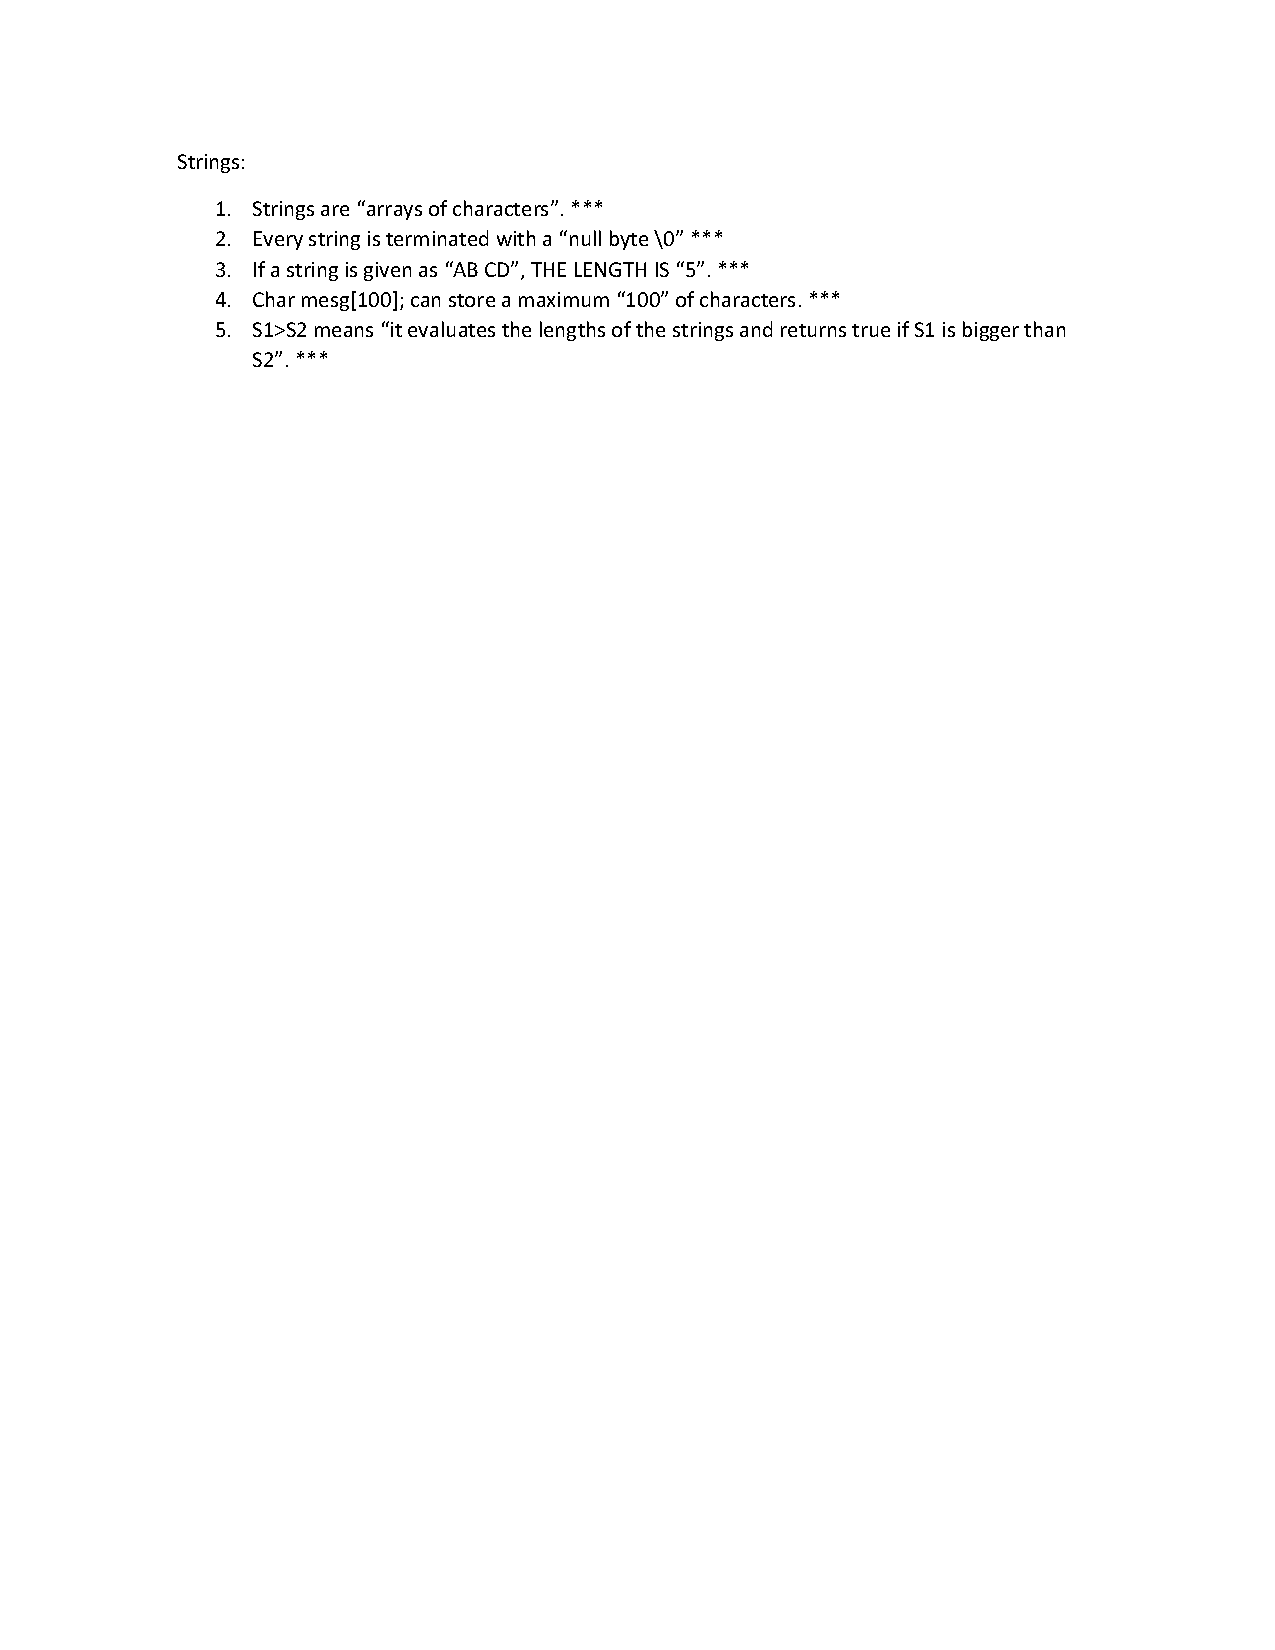
\includepdf[pages=-,pagecommand={\thispagestyle{plain}}]{Clases/00_EjercicioEnClase.pdf}
\section{Ejemplo del coronavirus}
\begin{itemize}
    \item Que las personas infectadas del coronavirus se mueran:
        \[
          P(\text{  Morir  }|\text{  Estoy\_enfemo  }) = \frac{\overbrace{42,000}^{\text{  Si esto sube el porcentage sube  }}}{60,000} = 0.03
        \]
    
\end{itemize}


%%%%%%%%%%%%%%%%%%%%%%%%%%%%%%%%%%%%%%%%%%%%%%%%%%%%%%%%%%%%%%%%%%%%%%%%%%%%%%%%%%%%%%%%%%%%%%%%%%%


\chapter{Clase - 2020-02-17}
\section{Las cuatro p's del marketing}
\begin{itemize}
    \item Producto 
    \item Precio 
    \item Plaza 
    \item Promoción 
    \item[*quinta p] posicionamiento 
\end{itemize}


%%%%%%%%%%%%%%%%%%%%%%%%%%%%%%%%%%%%%%%%%%%%%%%%%%%%%%%%%%%%%%%%%%%%%%%%%%%%%%%%%%%%%%%%%%%%%%%%%%%
\section{Escoger una sola palabra}
\begin{itemize}
    \item Cuando uno asocia elementos a la marca ese elemento se tiene que resumir en una sola palabra. 
\end{itemize}


%%%%%%%%%%%%%%%%%%%%%%%%%%%%%%%%%%%%%%%%%%%%%%%%%%%%%%%%%%%%%%%%%%%%%%%%%%%%%%%%%%%%%%%%%%%%%%%%%%%
\section{Palabras clave}
\begin{itemize}
    \item El posicionamiento tiende a funcionar si te anclas a un sentimiento profundo.
    \item Job to be done, Clayton Christensen.
\end{itemize}


\chapter{Clase - 2020-02-19}
\section{Linked list implemented with Stack}
\begin{itemize}
    \item List:
        \begin{itemize}
            \item Insert 
            \item Search/Traverse 
            \item Delete 
        \end{itemize}
    
    \item Stack:
        \begin{itemize}
            \item Push: insert on top 
            \item Pop: extract last inserted item 
            \item Peek: who is on top 
            \item Clear: empty stack
        \end{itemize}
    
    \item Una interfaz lo que define que contrato de implementación se tiene.
    \item Opcional: por que hace sentido que la clase stack extienda de vector.
\end{itemize}



\end{document}
